% !TEX TS-program = lualatex
\documentclass[a4paper,12pt,twoside,extrafontsizes]{memoir}

\usepackage{microtype}
\usepackage{alltt}
\usepackage{amsmath}
\usepackage[charter]{mathdesign}

\usepackage{fontspec}
\setmainfont[Ligatures=TeX]{XCharter}
\setmonofont[Scale=MatchLowercase]{DejaVu Sans Mono}

\usepackage[english]{babel}

\usepackage[perpage]{footmisc}

\newcommand{\styledtitleref}[1]{\emph{\titleref{#1}}}

%%%%%%%%%%%%%%%%%%%%%%%%%%%%%%%%%%
% Various Memoir class settings
%%%%%%%%%%%%%%%%%%%%%%%%%%%%%%%%%%

\sloppybottom
\setsecnumdepth{section}
\settocdepth{section}

\setpnumwidth{2.55em}
\setrmarg{3.55em}

%%%%%%%%%%%%%%%%%%%%%%%%%%%%%%%%%%
% Code
%%%%%%%%%%%%%%%%%%%%%%%%%%%%%%%%%%

\newcommand{\shellcmd}[1]{\texttt{#1}}
\newcommand{\code}[1]{\mbox{\texttt{#1}}}
\newcommand{\instr}[1]{\texttt{\textbf{#1}}}
\newcommand{\instrname}[1]{\emph{#1}}
\newcommand{\signal}[1]{\texttt{#1}}

\newenvironment{codepar}{%
	\vspace{0.5\baselineskip}%
	\begin{minipage}{0.9\textwidth}\begin{alltt}
}{%
	\end{alltt}\end{minipage}%
	\vspace{0.5\baselineskip}
}

\newenvironment{codeparbreakable}{%
	\vspace{0.5\baselineskip}%
	\begin{alltt}
		}{%
	\end{alltt}%
	\vspace{0.5\baselineskip}
}

%%%%%%%%%%%%%%%%%%%%%%%%%%%%%%%%%%
% Tables
%%%%%%%%%%%%%%%%%%%%%%%%%%%%%%%%%%

\newcolumntype{L}{>{\raggedright\arraybackslash}X}
\newcolumntype{R}{>{\raggedleft\arraybackslash}X}
\newcolumntype{C}{>{\centering\arraybackslash}X}

\newcolumntype{Q}[1]{>{\raggedright\arraybackslash}m{#1}}
\newcolumntype{E}[1]{>{\raggedleft\arraybackslash}m{#1}}
\newcolumntype{W}[1]{>{\centering\arraybackslash}m{#1}}

\newcommand{\tabcutin}[2]{\multicolumn{#1}{c}{\emph{#2}}}

%%%%%%%%%%%%%%%%%%%%%%%%%%%%%%%%%%
% Various stuff
%%%%%%%%%%%%%%%%%%%%%%%%%%%%%%%%%%

\newcommand{\cplusplus}{C\texttt{\raisebox{0.05em}{++}}}
\newcommand{\lxp}{\textls[60]{LXP}32}
\newcommand{\tocitem}[2]{\phantomsection\addcontentsline{toc}{#1}{#2}}

%%%%%%%%%%%%%%%%%%%%%%%%%%%%%%%%%%
% Hyperlinks
%%%%%%%%%%%%%%%%%%%%%%%%%%%%%%%%%%

\usepackage[bookmarks=true,
	bookmarksnumbered=true,
	bookmarksdepth=2,
	hypertexnames=false]
	{hyperref}

\hypersetup{
	pdftitle={LXP32 Technical Reference Manual},
	pdfauthor={Alex I. Kuznetsov}
}


\begin{document}

\frontmatter

% Title page

\thispagestyle{empty}
\pdfbookmark{Title}{bmk:title}
\calccentering{\unitlength}
\begin{adjustwidth*}{\unitlength}{-\unitlength}
	\vspace*{\fill}
	\begin{center}
	\DoubleSpacing
	
\includegraphics[scale=0.2]{images/lxp32-logo.pdf}\par
	\vspace{\onelineskip}
	\huge \lxp{}\par
	\Large a lightweight open source 32-bit CPU core\par
	\LARGE \textbf{Technical Reference Manual}\par
	\vspace{1.2\onelineskip}
	\large Version 1.1\par
	\vspace*{4\onelineskip}
	\end{center}
	\vspace*{\fill}
\end{adjustwidth*}

\clearpage

% Copyright page

\thispagestyle{empty}

{
\small
\setlength{\parindent}{0pt}
\nonzeroparskip

\vspace*{\fill}

Copyright \textcopyright{} 2016--2019 by Alex I. Kuznetsov.

The entire \lxp{} IP core package, including the synthesizable RTL description, verification environment, documentation and software tools, is distributed under the terms of the MIT license reproduced below:

Permission is hereby granted, free of charge, to any person obtaining a copy of this software and associated documentation files (the ``Software''), to deal in the Software without restriction, including without limitation the rights to use, copy, modify, merge, publish, distribute, sublicense, and/or sell copies of the Software, and to permit persons to whom the Software is furnished to do so, subject to the following conditions:

The above copyright notice and this permission notice shall be included in all copies or substantial portions of the Software.

THE SOFTWARE IS PROVIDED ``AS IS'', WITHOUT WARRANTY OF ANY KIND, EXPRESS OR IMPLIED, INCLUDING BUT NOT LIMITED TO THE WARRANTIES OF MERCHANTABILITY, FITNESS FOR A PARTICULAR PURPOSE AND NONINFRINGEMENT. IN NO EVENT SHALL THE AUTHORS OR COPYRIGHT HOLDERS BE LIABLE FOR ANY CLAIM, DAMAGES OR OTHER LIABILITY, WHETHER IN AN ACTION OF CONTRACT, TORT OR OTHERWISE, ARISING FROM, OUT OF OR IN CONNECTION WITH THE SOFTWARE OR THE USE OR OTHER DEALINGS IN THE SOFTWARE.

\vspace{4\baselineskip}

Mentor Graphics and ModelSim are trademarks of Mentor Graphics Corporation.

Microsemi and IGLOO are trademarks of Microsemi Corporation.

Microsoft, Windows and Visual Studio are either registered trademarks or trademarks of Microsoft Corporation in the United States and/or other countries.

Verilog is a registered trademark of Cadence Design Systems, Inc.

Xilinx, Artix and Vivado are trademarks of Xilinx in the United States and other countries.

All other trademarks are the property of their respective owners.
}

\cleardoublepage

% Table of contents

\pdfbookmark{\contentsname}{bmk:contents}

\tableofcontents*


\mainmatter

\chapter{Introduction}

\section{Main features}

\lxp{} (\emph{Lightweight eXecution Pipeline}) is a small 32-bit CPU IP core optimized for FPGA implementation. Its key features include:

\begin{itemize}
	\item portability (described in behavioral VHDL-93, not tied to any particular vendor);
	\item 3-stage hazard-free pipeline;
	\item 256 registers implemented as a RAM block;
	\item a simple instruction set with only 30 distinct opcodes;
	\item separate instruction and data buses, optional instruction cache;
	\item WISHBONE compatibility;
	\item 8 interrupts with hardwired priorities;
	\item optional divider.
\end{itemize}

As a lightweight CPU core, \lxp{} lacks some features of more advanced processors, such as nested interrupt handling, debugging support, floating-point and memory management units. \lxp{} is based on an original ISA (Instruction Set Architecture) which does not currently have a C compiler. It can be programmed in the assembly language covered by Appendix \ref{app:assemblylanguage}.

Two major hardware versions of the CPU are provided: \lxp{}U which does not include an instruction cache and uses the Low Latency Interface (Section \ref{sec:lli}) to fetch instructions, and \lxp{}C which fetches instructions over a cached WISHBONE bus protocol. These versions are otherwise identical and have the same instruction set architecture.

\section{Implementation estimates}

Typical results of \lxp{} core FPGA implementation are presented in Table \ref{tab:implementation}. Note that these data are only useful as rough estimates, since actual results depend greatly on tool versions and configuration, design constraints, device utilization ratio and other factors.

Data on two configurations are provided:

\begin{itemize}
	\item \emph{Compact}: \lxp{}U (without instruction cache), no divider, 2-cycle multiplier.
	\item \emph{Full}: \lxp{}C (with instruction cache), divider, 2-cycle multiplier.
\end{itemize}

The slowest speed grade was used for clock frequency estimation.

\begin{table}[htbp]
	\caption{Typical results of \lxp{} core FPGA implementation}
	\label{tab:implementation}
	\begin{tabularx}{\textwidth}{Q{0.5\textwidth}LL}
		\toprule
		Resource & Compact & Full \\
		\midrule
		\multicolumn{3}{c}{Microsemi\textregistered{} IGLOO\textregistered{}2 M2GL005-FG484} \\
		\midrule
		Logic elements (LUT+DFF) & 1457 & 2086 \\
		\hspace*{1em}LUTs & 1421 & 1999 \\
		\hspace*{1em}Flip-flops & 706 & 1110 \\
		Mathblocks (MACC) & 3 & 3 \\
		RAM blocks (RAM1K18) & 2 & 3 \\
		Clock frequency & 107.7 MHz & 109.2 MHz \\
		\midrule
		\multicolumn{3}{c}{Xilinx\textregistered{} Artix\textregistered{}-7 xc7a15tfgg484-1} \\
		\midrule
		Slices & 235 & 365 \\
		\hspace*{1em}LUTs & 666 & 1011 \\
		\hspace*{1em}Flip-flops & 528 & 883 \\
		DSP blocks (DSP48E1) & 4 & 4 \\
		RAM blocks (RAMB18E1) & 2 & 3 \\
		Clock frequency & 111.9 MHz & 120.2 MHz \\
		\bottomrule
	\end{tabularx}
\end{table}

\section{Structure of this manual}

General description of the \lxp{} operation from a software developer's point of view can be found in Chapter \ref{ch:isa}, \styledtitleref{ch:isa}. Future versions of the \lxp{} CPU are intended to be at least backwards compatible with this architecture.

Topics related to hardware, such as synthesis, implementation and interfacing other IP cores, are covered in Chapter \ref{ch:integration}, \styledtitleref{ch:integration}. A brief description of the \lxp{} pipelined architecture is provided in Chapter \ref{ch:pipeline}, \styledtitleref{ch:pipeline}. The \lxp{} IP core package includes a verification environment (self-checking testbench) which can be used to simulate the design as described in Chapter \ref{ch:simulation}, \styledtitleref{ch:simulation}.

Documentation for tools shipped with the \lxp{} IP core package (assembler/linker, disassembler and interconnect generator) is provided in Chapter \ref{ch:developmenttools}, \styledtitleref{ch:developmenttools}.

Appendices include a detailed description of the \lxp{} instruction set, instruction cycle counts and \lxp{} assembly language definition. WISHBONE datasheet required by the WISHBONE specification is also provided.

\chapter{Instruction set architecture}
\label{ch:isa}

\section{Data format}

Most \lxp{} instructions work with 32-bit data words. A few instructions that address individual bytes use little-endian order, that is, the least significant byte is stored at the lowest address. Signed values are encoded in a 2's complement format.

\section{Instruction format}
\label{sec:instructionformat}

All \lxp{} instructions are encoded as 32-bit words, with the exception of \instr{lc} (\instrname{Load Constant}), which occupies two adjacent 32-bit words. Instructions in memory must be aligned to word boundaries.

Most arithmetic and logical instructions take two source operands and write the result to an independent destination register. General instruction format is presented on Figure \ref{fig:instructionformat}.

\begin{figure}[htbp]
	\centering
	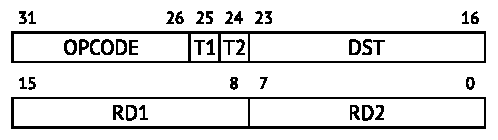
\includegraphics[scale=1.2]{images/instructionformat.pdf}
	\caption{\lxp{} instruction format}
	\label{fig:instructionformat}
\end{figure}

This format includes the following fields:

\begin{enumerate}
	\item OPCODE -- a 6-bit instruction code (see Appendix \ref{app:instructionset}).
	\item T1 -- type of the RD1 field.
	\item T2 -- type of the RD2 field.
	\item DST -- register number (usually the destination register).
	\item RD1 -- register/direct operand 1.
	\item RD2 -- register/direct operand 2.
\end{enumerate}

Some of these fields may not have meaning for a particular instruction; such unused fields are replaced with zeros.

DST field specifies one of the 256 \lxp{} registers. RD1 and RD2 fields can denote either source register operands or direct (immediate) operands: if the corresponding T field is 1, RD value is a register number, otherwise it is interpreted as a direct signed byte in a 2's complement format (valid values range from -128 to 127).

For example, consider the following instruction that adds \code{10} to \code{r0} and writes the result to \code{r1}:

\begin{codepar}
    \instr{add} r1, r0, 10
\end{codepar}

In this example, OPCODE is \code{010000}, T1 is \code{1}, T2 is \code{0}, DST is \code{00000001}, RD1 is \code{00000000} and RD2 is \code{00001010}. Hence, the instruction is encoded as \code{0x4201000A}.

For convenience, some instructions have alias mnemonics. For example, \lxp{} does not have a distinct \instr{mov} opcode: instead, \code{\instr{mov} dst, src} is an alias for \code{\instr{add} dst, src, 0}.

A complete list of \lxp{} instructions is provided in Appendix \ref{app:instructionset}.

\section{Registers}

\lxp{} has 256 registers denoted as \code{r0} -- \code{r255}. The first 240 of them (from \code{r0} to \code{r239}) are general-purpose registers (GPR), the last 16 (from \code{r240} to \code{r255}) are special-purpose registers (SPR). For convenience, some special-purpose registers have alias names: for example, \code{r255} can be also referred to as \code{sp} (stack pointer). Special purpose registers are listed in Table \ref{tab:spr}. Some of these registers are reserved: the software should not access them.

\begin{table}[htbp]
	\caption{\lxp{} special-purpose registers}
	\label{tab:spr}
	\begin{tabularx}{\textwidth}{llL}
		\toprule
		Alias name & Generic name & Description \\
		\midrule
		\code{iv0} & \code{r240} & Interrupt vector 0 (Section \ref{sec:interrupthandling}) \\
		\code{iv1} & \code{r241} & Interrupt vector 1 (Section \ref{sec:interrupthandling}) \\
		\code{iv2} & \code{r242} & Interrupt vector 2 (Section \ref{sec:interrupthandling}) \\
		\code{iv3} & \code{r243} & Interrupt vector 3 (Section \ref{sec:interrupthandling}) \\
		\code{iv4} & \code{r244} & Interrupt vector 4 (Section \ref{sec:interrupthandling}) \\
		\code{iv5} & \code{r245} & Interrupt vector 5 (Section \ref{sec:interrupthandling}) \\
		\code{iv6} & \code{r246} & Interrupt vector 6 (Section \ref{sec:interrupthandling}) \\
		\code{iv7} & \code{r247} & Interrupt vector 7 (Section \ref{sec:interrupthandling}) \\
		\multicolumn{1}{l}{---} & \code{r248}\,--\,\code{r251} & \emph{Reserved} \\
		\code{cr}  & \code{r252} & Control register (Section \ref{sec:interrupthandling}) \\
		\code{irp} & \code{r253} & Interrupt return pointer (Section \ref{sec:interrupthandling}) \\
		\code{rp}  & \code{r254} & Return pointer (Section \ref{sec:callingprocedures})\\
		\code{sp}  & \code{r255} & Stack pointer (Section \ref{sec:stack}) \\
		\bottomrule
	\end{tabularx}
\end{table}

All registers are zero-initialized during the CPU reset.

\section{Addressing}
\label{sec:addressing}

All addressing in \lxp{} is indirect. In order to access a memory location, its address must be stored in a register; any available register can be used for this purpose.

Some instructions, namely \instr{lsb} (\instrname{Load Signed Byte}), \instr{lub} (\instrname{Load Unsigned Byte}) and \instr{sb} (\instrname{Store Byte}) provide byte-granular access, in which case all 32 bits in the address are significant. Otherwise the least two address bits are ignored as \lxp{} doesn't support unaligned access to 32-bit data words (during simulation, a warning is emitted if such a transaction is attempted).

A special rule applies to pointers that refer to instructions: since instructions are always word-aligned, the least significant bit is interpreted as the \code{IRF} (\emph{Interrupt Return Flag}). See Section \ref{sec:interrupthandling} for details.

\section{Stack}
\label{sec:stack}

The current pointer to the top of the stack is stored in the \code{sp} register. To the hardware this register is not different from general purpose registers, that is, in no situation does the CPU access the stack implicitly (procedure calls and interrupts use register-based conventions).

Software can access the stack as follows:

\begin{codepar}
    \emph{// push r0 on the stack}
    \instr{sub} sp, sp, 4
    \instr{sw} sp, r0
    \emph{// pop r0 from the stack}
    \instr{lw} r0, sp
    \instr{add} sp, sp, 4
\end{codepar}

Before using the stack, the \code{sp} register must be set up to point to a valid memory location. The simplest software can operate stackless, or even without data memory altogether if registers are enough to store the program state.

\section{Calling procedures}
\label{sec:callingprocedures}

\lxp{} provides a \instr{call} instruction which saves the address of the next instruction in the \code{rp} register and transfers execution to the address stored in the register operand. Return from a procedure is performed by the \code{\instr{jmp} rp} instruction which also has a \instr{ret} alias.

If a procedure must in turn call a nested procedure itself, the return address in the \code{rp} register will be overwritten by the \instr{call} instruction. Hence, unless it is a tail call (see below), the procedure must save the \code{rp} value somewhere; the most general solution is to use the stack:

\begin{codepar}
    \instr{sub} sp, sp, 4
    \instr{sw} sp, rp
    ...
    \instr{lc} r0, Nested_proc
    \instr{call} r0
    ...
    \instr{lw} rp, sp
    \instr{add} sp, sp, 4
    \instr{ret}
\end{codepar}

Procedures that don't use the \instr{call} instruction (sometimes called \emph{leaf procedures}) don't need to save the \code{rp} value.

Since \instr{ret} is just an alias for \code{\instr{jmp} rp}, one can also use \instrname{Compare and Jump} instructions (\instr{cjmp\emph{xxx}}) to perform a conditional procedure return. For example, consider the following procedure which calculates the absolute value of \code{r1}:

\begin{codepar}
Abs_proc:
    \instr{cjmpsge} rp, r1, 0 \emph{// return immediately if r1>=0}
    \instr{neg} r1, r1 \emph{// otherwise, negate r1}
    \instr{ret} \emph{// jmp rp}
\end{codepar}

A \emph{tail call} is a special type of procedure call where the calling procedure calls a nested procedure as the last action before return. In such cases the \instr{call} instruction can be replaced with \instr{jmp}, so that when the nested procedure executes \instr{ret}, it returns directly to the caller's parent procedure.

Although the \lxp{} architecture doesn't mandate any particular calling convention, some general recommendations are presented below:

\begin{enumerate}
	\item Pass arguments and return values through the \code{r1}--\code{r31} registers (a procedure can have multiple return values).
	\item If necessary, the \code{r0} register can be used to load the procedure address.
	\item Designate \code{r0}--\code{r31} registers as \emph{caller-saved}, that is, they are not guaranteed to be preserved during procedure calls and must be saved by the caller if needed. The procedure can use them for any purpose, regardless of whether they are used to pass arguments and/or return values.
\end{enumerate}

\section{Interrupt handling}
\label{sec:interrupthandling}

\subsection{Control register}

\lxp{} supports 8 interrupts with hardwired priority levels (interrupts with lower vector numbers have higher priority). Interrupts vectors (pointers to interrupt handlers) are stored in the \code{iv0}--\code{iv7} registers. Interrupt handling is controlled by the \code{cr} register (Table \ref{tab:cr}).

\begin{table}[htbp]
	\caption{Control register}
	\label{tab:cr}
	\begin{tabularx}{\textwidth}{lL}
		\toprule
		Bit & Description \\
		\midrule
		0      & Enable interrupt 0 \\
		1      & Enable interrupt 1 \\
		& \ldots \\
		7      & Enable interrupt 7 \\
		8      & Temporarily block interrupt 0 \\
		9      & Temporarily block interrupt 1 \\
		& \ldots \\
		15     & Temporarily block interrupt 7 \\
		31--16 & \emph{Reserved} \\
		\bottomrule
	\end{tabularx}
\end{table}

Disabled interrupts are ignored altogether: if the CPU receives an interrupt request signal while the corresponding interrupt is disabled, the interrupt handler will not be called even if the interrupt is enabled later. Conversely, temporarily blocked interrupts are still registered, but their handlers are not called until they are unblocked.

Like other registers, \code{cr} is zero-initialized during the CPU reset, meaning that no interrupts are initially enabled.

\subsection{Invoking interrupt handlers}

Interrupt handlers are invoked by the CPU similarly to procedures (Section \ref{sec:callingprocedures}), the difference being that in this case return address is stored in the \code{irp} register (as opposed to \code{rp}), and the least significant bit of the register (\code{IRF} -- \emph{Interrupt Return Flag}) is set.

An interrupt handler returns using the \code{\instr{jmp} irp} instruction which also has an \instr{iret} alias. Until the interrupt handler returns, the CPU will defer further interrupt processing (although incoming interrupt requests will still be registered). This also means that the \code{irp} register value will not be unexpectedly overwritten. When executing the \code{\instr{jmp} irp} instruction, the CPU will recognize the \code{IRF} flag and resume interrupt processing as usual. It is also possible to perform a conditional return from the interrupt handler, similarly to the technique described in Section \ref{sec:callingprocedures} for conditional procedure returns.

\subsection{Non-returnable interrupts}

If an interrupt vector has the least significant bit (\code{IRF}) set, the CPU will resume interrupt processing immediately. One should not try to invoke \instr{iret} from such a handler since the \code{irp} register could have been overwritten by another interrupt. This technique can be useful when the CPU's only task is to process external events:

\begin{codeparbreakable}
\emph{// Set the IRF to mark the interrupt as non-returnable}
    \instr{lc} iv0, main\_loop@1
    \instr{mov} cr, 1 \emph{// enable the interrupt}
    \instr{hlt} \emph{// wait for an interrupt request}
main\_loop:
\emph{// Process the event...}
    \instr{hlt} \emph{// wait for the next interrupt request}
\end{codeparbreakable}

Note that \instr{iret} is never called in this example.

\chapter{Integration}
\label{ch:integration}

\section{Overview}

The \lxp{} IP core is delivered in a form of a synthesizable RTL description expressed in \mbox{VHDL-93}. It does not use any technology specific primitives and should work out of the box with major FPGA synthesis software. \lxp{} can be integrated in both VHDL and Verilog\textregistered{} based SoC designs.

Major \lxp{} hardware versions have separate top-level design units:

\begin{itemize}
	\item \shellcmd{lxp32u\_top} -- \lxp{}U (without instruction cache),
	\item \shellcmd{lxp32c\_top} -- \lxp{}C (with instruction cache).
\end{itemize}

A high level block diagram of the CPU is presented on Figure \ref{fig:blockdiagram}. Schematic symbols for \lxp{}U and \lxp{}C are shown on Figure \ref{fig:symbols}.

\begin{figure}[htbp]
	\centering
	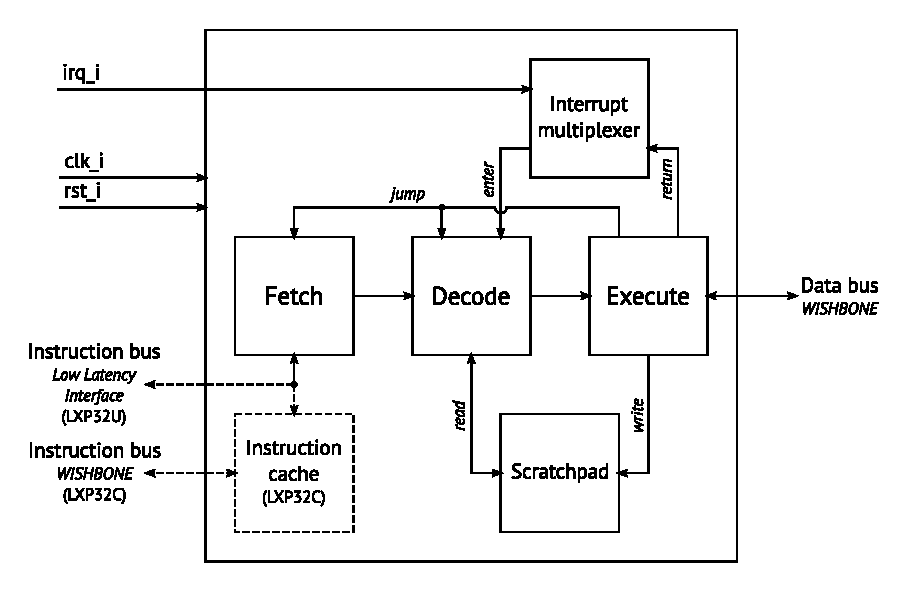
\includegraphics[scale=0.85]{images/blockdiagram.pdf}
	\caption{\lxp{} CPU block diagram}
	\label{fig:blockdiagram}
\end{figure}

\begin{figure}[htbp]
	\centering
	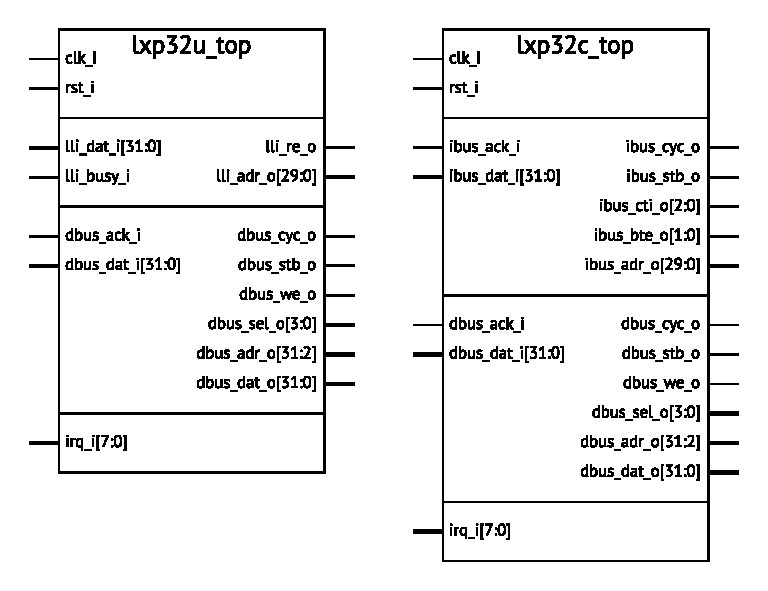
\includegraphics[scale=0.85]{images/symbols.pdf}
	\caption{Schematic symbols for \lxp{}U and \lxp{}C}
	\label{fig:symbols}
\end{figure}

\lxp{}U uses the Low Latency Interface (LLI) described in Section \ref{sec:lli} to fetch instructions. This interface is designed to interact with low latency on-chip peripherals such as RAM blocks. It works best with slaves that can return the instruction on the next cycle after its address has been set, although the slave can still introduce wait states if needed. Low Latency Interface can be also connected to a custom (external) instruction cache.

To achieve the least possible latency, some LLI outputs are not registered. For this reason the LLI is not suitable for interaction with off-chip peripherals.

\lxp{}C is designed to work with high latency memory controllers and uses a simple instruction cache based on a ring buffer. The instructions are fetched over the WISHBONE instruction bus. To maximize throughput, the CPU makes use of the WISHBONE registered feedback signals [CTI\_O()] and [BTE\_O()]. All outputs on this bus are registered. This version is also recommended for use in situations where LLI combinatorial delays are unacceptable.

Both \lxp{}U and \lxp{}C use the WISHBONE protocol for the data bus.

\section{Ports}

\begin{ctabular}{lccl}
	\toprule
	Port & Direction & Bus width & Description \\
	\midrule
	\tabcutin{4}{Global signals} \\
	\midrule
	\signal{clk\_i} & in & 1 & System clock \\
	\signal{rst\_i} & in & 1 & Synchronous reset, active high \\
	\midrule
	\tabcutin{4}{Instruction bus -- Low Latency Interface (\lxp{}U only)} \\
	\midrule
	\signal{lli\_re\_o} & out & 1 & Read enable output, active high \\
	\signal{lli\_adr\_o} & out & 30 & Address output \\
	\signal{lli\_dat\_i} & in & 32 & Data input \\
	\signal{lli\_busy\_i} & in & 1 & Busy flag input, active high \\
	\midrule
	\tabcutin{4}{Instruction bus -- WISHBONE (\lxp{}C only)} \\
	\midrule
	\signal{ibus\_cyc\_o} & out & 1 & Cycle output \\
	\signal{ibus\_stb\_o} & out & 1 & Strobe output \\
	\signal{ibus\_cti\_o} & out & 3 & Cycle type identifier \\
	\signal{ibus\_bte\_o} & out & 2 & Burst type extension \\
	\signal{ibus\_ack\_i} & in & 1 & Acknowledge input \\
	\signal{ibus\_adr\_o} & out & 30 & Address output \\
	\signal{ibus\_dat\_i} & in & 32 & Data input \\
	\midrule
	\tabcutin{4}{Data bus} \\
	\midrule
	\signal{dbus\_cyc\_o} & out & 1 & Cycle output \\
	\signal{dbus\_stb\_o} & out & 1 & Strobe output \\
	\signal{dbus\_we\_o} & out & 1 & Write enable output \\
	\signal{dbus\_sel\_o} & out & 4 & Select output \\
	\signal{dbus\_ack\_i} & in & 1 & Acknowledge input \\
	\signal{dbus\_adr\_o} & out & 30 & Address output \\
	\signal{dbus\_dat\_o} & out & 32 & Data output \\
	\signal{dbus\_dat\_i} & in & 32 & Data input \\
	\midrule
	\tabcutin{4}{Other ports} \\
	\midrule
	\signal{irq\_i} & in & 8 & Interrupt requests \\
	\bottomrule
\end{ctabular}

\section{Generics}
\label{sec:generics}

The following generics can be used to configure the \lxp{} IP core parameters.

\subsection{DBUS\_RMW}

By default, \lxp{} uses the \signal{dbus\_sel\_o} (byte enable) port to perform byte-granular write transactions initiated by the \instr{sb} (\instrname{Store Byte}) instruction. If this option is set to \code{true}, \signal{dbus\_sel\_o} is always tied to \code{"1111"}, and byte-granular write access is performed using the RMW (read-modify-write) cycle. The latter method is slower, but can work with slaves that do not have the [SEL\_I()] port.

This feature is designed with the assumption that read and write transactions do not cause side effects, thus it can be unsuitable for some slaves.

\subsection{DIVIDER\_EN}

\lxp{} includes a divider unit which has quite a low performance but occupies a considerable amount of resources. It can be disabled by setting this option to \code{false}.

\subsection{IBUS\_BURST\_SIZE}

Instruction bus burst size. Default value is 16. Only for \lxp{}C.

\subsection{IBUS\_PREFETCH\_SIZE}

Number of words that the instruction cache will read ahead from the current instruction pointer. Default value is 32. Only for \lxp{}C.

\subsection{MUL\_ARCH}

\lxp{} provides three multiplier options:

\begin{itemize}
	\item \code{"dsp"} is the fastest architecture designed for technologies that provide fast parallel $16 \times 16$ multipliers, which includes most modern FPGA families. One multiplication takes 2 clock cycles.
	\item \code{"opt"} architecture uses a semi-parallel multiplication algorithm based on carry-save accumulation of partial products. It is designed for technologies that do not provide fast $16 \times 16$ multipliers. One multiplication takes 6 clock cycles.
	\item \code{"seq"} is a fully sequential design. One multiplication takes 34 clock cycles.
\end{itemize}

The default multiplier architecture is \code{"dsp"}. This option is recommended for most modern FPGA devices regardless of optimization goal since it is not only the fastest, but also occupies the least amount of general-purpose logic resources. However, it will create a timing bottleneck on technologies that lack fast multipliers.

For older FPGA families that don't provide dedicated multipliers the \code{"opt"} architecture can be used if decent throughput is still needed. It is designed to avoid creating a timing bottleneck on such technologies. Alternatively, \code{"seq"} architecture can be used when throughput is not a concern.

\subsection{START\_ADDR}

Address of the first instruction to be executed after CPU reset. Default value is \code{0}. The two least significant bits are ignored as instructions are always word-aligned.

\section{Clock and reset}
\label{sec:clockreset}

All flip-flops in the CPU are triggered by a rising edge of the \signal{clk\_i} signal. No specific requirements are imposed on the \signal{clk\_i} signal apart from usual constraints on setup and hold times.

\lxp{} is reset synchronously when the \signal{rst\_i} signal is asserted. If the system reset signal comes from an asynchronous source, a synchronization circuit must be used; an example of such a circuit is shown on Figure \ref{fig:resetsync}.

\begin{figure}[htbp]
	\centering
	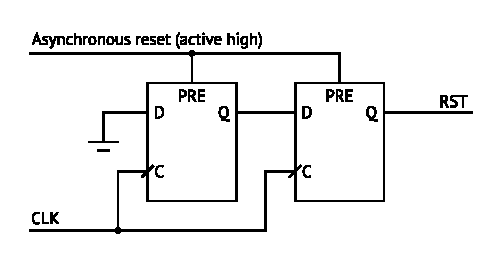
\includegraphics[scale=1]{images/resetsync.pdf}
	\caption{Reset synchronization circuit}
	\label{fig:resetsync}
\end{figure}

In SRAM-based FPGAs flip-flops and RAM blocks have deterministic state after a bitstream is loaded. On such technologies \lxp{} can operate without reset. In this case the \signal{rst\_i} port can be tied to a logical \code{0} in the RTL design to allow the synthesizer to remove redundant logic.

\signal{clk\_i} and \signal{rst\_i} signals also serve the role of [CLK\_I] and [RST\_I] WISHBONE signals, respectively, for both instruction and data buses.

\section{Low Latency Interface}
\label{sec:lli}

Low Latency Interface (LLI) is a simple pipelined synchronous protocol with a typical latency of 1 cycle used by \lxp{}U to fetch instructions. It was designed to allow simple connection of the CPU to on-chip program RAM or cache. The timing diagram of the LLI is shown on Figure \ref{fig:llitiming}.

\begin{figure}[htbp]
	\centering
	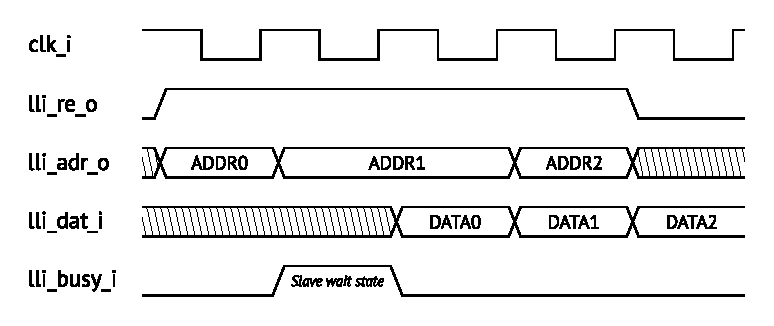
\includegraphics[scale=1]{images/llitiming.pdf}
	\caption{Low Latency Interface timing diagram (\lxp{}U)}
	\label{fig:llitiming}
\end{figure}

To request a word, the master produces its address on \signal{lli\_adr\_o} and asserts \signal{lli\_re\_o}. The request is considered valid when \signal{lli\_re\_o} is high and \signal{lli\_busy\_i} is low on the same clock cycle. On the next cycle after a valid request, the slave must either produce data on \signal{lli\_dat\_i} or assert \signal{lli\_busy\_i} to indicate that data are not ready. \signal{lli\_busy\_i} must be held high until the valid data are present on the \signal{lli\_dat\_i} port.

The data provided by the slave are only required to be valid on the next cycle after a valid request (if \signal{lli\_busy\_i} is not asserted) or on the cycle when \signal{lli\_busy\_i} is deasserted after being held high. Otherwise \signal{lli\_dat\_i} is undefined.

The values of \signal{lli\_re\_o} and \signal{lli\_adr\_o} are not guaranteed to be preserved by the master while the slave is busy.

The simplest slaves such as on-chip RAM blocks which are never busy can be trivially connected to the LLI by connecting address, data and read enable ports and tying the \signal{lli\_busy\_i} signal to a logical \code{0} (you can even ignore \signal{lli\_re\_o} in this case, although doing so can theoretically increase power consumption).

Note that the \signal{lli\_adr\_o} signal has a width of 30 bits since it addresses words, not bytes (instructions are always word-aligned).

Since the \signal{lli\_re\_o} output signal is not registered, this interface is not suitable for interaction with off-chip peripherals. Also, care should be taken to avoid introducing too much additional combinatorial delay on its outputs.

\section{WISHBONE instruction bus}

The \lxp{}C CPU fetches instructions over the WISHBONE bus. Its parameters are defined in the WISHBONE datasheet (Appendix \ref{app:wishbonedatasheet}). For a detailed description of the bus protocol refer to the WISHBONE specification, revision B3.

With classic WISHBONE handshake decent throughput can be only achieved when the slave is able to terminate cycles asynchronously. It is usually possible only for the simplest slaves which should probably be using the Low Latency Interface instead. To maximize throughput for complex, high latency slaves, \lxp{}C instruction bus uses optional WISHBONE address tags [CTI\_O()] (Cycle Type Identifier) and [BTE\_O()] (Burst Type Extension). These signals are hints allowing the slave to predict the address that will be set by the master in the next cycle and prepare data in advance. The slave can ignore these hints, processing requests as classic WISHBONE cycles, although performance would almost certainly suffer in this case.

A typical \lxp{}C instruction bus burst timing diagram is shown on Figure \ref{fig:ibustiming}.

\begin{figure}[htbp]
	\centering
	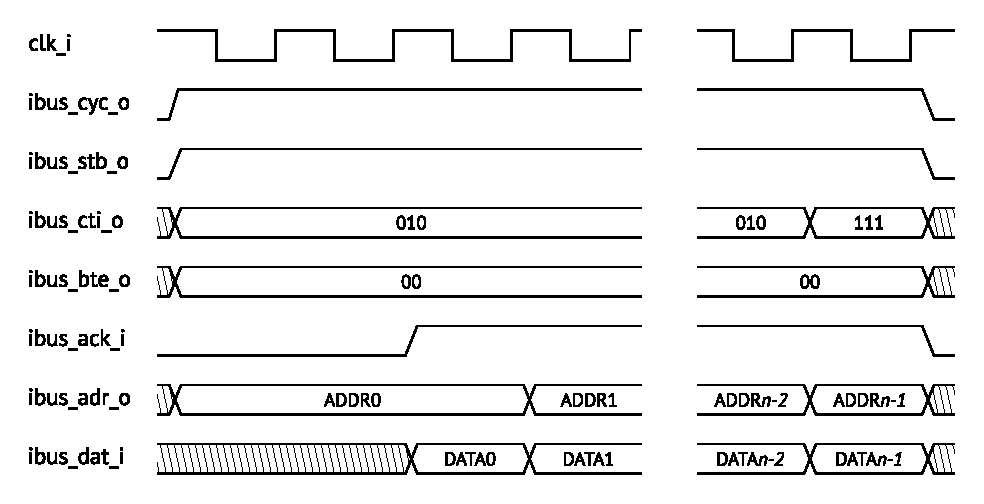
\includegraphics[scale=0.786]{images/ibustiming.pdf}
	\caption{Typical WISHBONE instruction bus burst (\lxp{}C)}
	\label{fig:ibustiming}
\end{figure}

\section{WISHBONE data bus}

\lxp{} uses the WISHBONE bus to interact with data memory and other peripherals. This bus is distinct from the instruction bus; its parameters are defined in the WISHBONE datasheet (Appendix \ref{app:wishbonedatasheet}).

This bus uses a 30-bit \signal{dbus\_adr\_o} port to address 32-bit words; the \signal{dbus\_sel\_o} port is used to select individual bytes to be written or read. Alternatively, with the \code{DBUS\_RMW} option (Section \ref{sec:generics}) the \signal{dbus\_sel\_o} port is not used; byte-granular write access is performed using the read-modify-write cycle instead.

For a detailed description of the bus protocol refer to the WISHBONE specification, revision B3.

Typical timing diagrams for write and read cycles are shown on Figure \ref{fig:dbustiming}. In these examples the peripheral terminates the cycle asynchronously; however, it can also introduce wait states by delaying the \signal{dbus\_ack\_i} signal.

\begin{figure}[htbp]
	\centering
	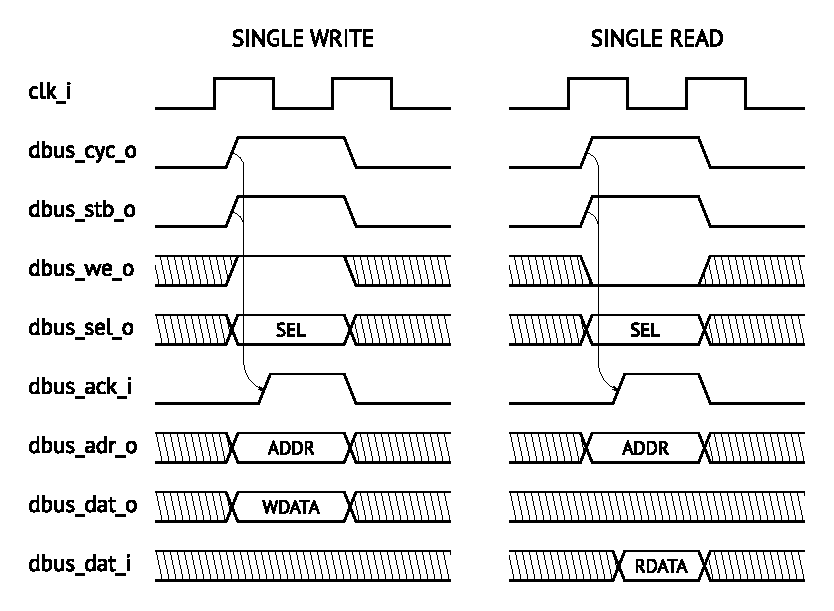
\includegraphics[scale=0.928]{images/dbustiming.pdf}
	\caption{Typical WISHBONE data bus WRITE and READ cycles}
	\label{fig:dbustiming}
\end{figure}

\section{Interrupts}

\lxp{} registers an interrupt condition when the corresponding request signal goes from \code{0} to \code{1}. Transitions from \code{1} to \code{0} are ignored. All interrupt request signals must be synchronous with the system clock (\signal{clk\_i}); if coming from an asynchronous source, they must be synchronized using a sequence of at least two flip-flops clocked by \signal{clk\_i}. These flip-flops are not included in the \lxp{} core in order not to increase interrupt processing delay for interrupt sources that are inherently synchronous. Failure to properly synchronize interrupt request signals will cause timing violations that will manifest itself as intermittent, hard to debug faults.

\section{Synthesis and optimization}
\label{sec:synthesis}

\subsection{Technology specific primitives}

\lxp{} RTL design is described in behavioral VHDL. However, it can also benefit from certain special resources provided by most FPGA devices, namely, RAM blocks and dedicated multipliers. For improved portability, hardware description that can potentially be mapped to such resources is localized in separate design units:

\begin{itemize}
	\item \shellcmd{lxp32\_ram256x32} -- a dual-port synchronous $256 \times 32$ bit RAM with one write port and one read port;
	\item \shellcmd{lxp32\_mul16x16} -- an unsigned $16 \times 16$ multiplier with an output register.
\end{itemize}

These design units contain behavioral description of respective hardware that is recognizable by FPGA synthesis tools. Usually no adjustments are needed as the synthesizer will automatically infer an appropriate primitive from its behavioral description. If automatic inference produces unsatisfactory results, these design units can be replaced with library element wrappers. The same is true for ASIC logic synthesis software which is unlikely to infer complex primitives.

\lxp{} implements its own bypass logic dealing with situations when RAM read and write addresses collide. It does not depend on the read/write conflict resolution behavior of the underlying primitive.

\subsection{General optimization guidelines}

This subsection contains general advice on achieving satisfactory synthesis results regardless of the optimization goal. Some of these suggestions are also mentioned in other parts of this manual.

\begin{enumerate}
	\item If the technology doesn't provide dedicated multiplier resources, consider using \code{"opt"} or \code{"seq"} multiplier architecture (Section \ref{sec:generics}).
	
	\item Ensure that the instruction bus has adequate throughput. For \lxp{}C, check that the slave supports the WISHBONE registered feedback signals [CTI\_I()] and [BTE\_I()].
	
	\item Multiplexing instruction and data buses, or connecting them to the same interconnect that allows only one master at a time to be active (i.e. \emph{shared bus} interconnect topology) is not recommended. If you absolutely must do so, assign a higher priority level to the data bus, otherwise instruction prefetches will massively slow down data transactions.
	
	\item For small programs, consider mapping code and data memory to the beginning or end of the address space (i.e. \code{0x00000000}--\code{0x000FFFFF} or \code{0xFFF00000}--\code{0xFFFFFFFF}) to be able to load pointers with the \instr{lcs} instruction which saves both memory and CPU cycles as compared to \instr{lc}.
\end{enumerate}

\subsection{Optimizing for timing}

\begin{enumerate}
	\item Set up reasonable timing constraints. Do not overconstrain the design by more than 10--15~\%.
	
	\item Analyze the worst path. The natural \lxp{} timing bottleneck usually goes from the scratchpad (register file) output through the ALU (in the Execute stage) to the scratchpad input. If timing analysis lists other critical paths, the problem can lie elsewhere. If the \signal{rst\_i} signal becomes a bottleneck, promote it to a global network or, with SRAM-based FPGAs, consider operating without reset (see Section \ref{sec:clockreset}). Critical paths affecting the WISHBONE state machines could indicate problems with interconnect performance.
	
	\item Configure the synthesis tool to reduce the fanout limit. Note that setting this limit to a too small value can lead to an opposite effect.
	
	\item Synthesis tools can support additional options to improve timing, such as the \emph{Retiming} algorithm which rearranges registers and combinatorial logic across the pipeline in attempt to balance delays. The efficiency of such algorithms is not very predictable. In general, sloppy designs are the most likely to benefit from it, while for a carefully designed circuit timing can sometimes get worse.
\end{enumerate}

\subsection{Optimizing for area}

\begin{enumerate}
	\item Consider disabling the divider if not using it (see Section \ref{sec:generics}).
	
	\item Relaxing timing constraints can sometimes allow the synthesizer to produce a more area-efficient circuit.
	
	\item Increase the fanout limit in the synthesizer settings to reduce buffer replication.
\end{enumerate}

\chapter{Hardware architecture}
\label{ch:pipeline}

The \lxp{} CPU is based on a 3-stage hazard-free pipelined architecture and uses a large RAM-based register file (scratchpad) with two read ports and one write port. The pipeline includes the following stages:

\begin{itemize}
	\item\emph{Fetch} -- fetches instructions from the program memory.
	\item\emph{Decode} -- decodes instructions and reads register operand values from the scratchpad.
	\item\emph{Execute} -- executes instructions and writes the results (if any) to the scratchpad.
\end{itemize}

\lxp{} instructions are encoded in such a way that operand register numbers can be known without decoding the instruction (Section \ref{sec:instructionformat}). When the \emph{Fetch} stage produces an instruction, scratchpad input addresses are set immediately, before the instruction itself is decoded. If the instruction does not use one or both of the register operands, the corresponding data read from the scratchpad are discarded. Collision bypass logic in the scratchpad detects situations where the \emph{Decode} stage tries to read a register which is currently being written by the \emph{Execute} stage and forwards its value, bypassing the RAM block and avoiding Read After Write (RAW) pipeline hazards. Other types of data hazards are also impossible with this architecture.

As an example, consider the following simple code chunk:

\begin{codepar}
    \instr{mov} r0, 10 \emph{// alias for add r0, 10, 0}
    \instr{mov} r1, 20 \emph{// alias for add r1, 20, 0}
    \instr{add} r2, r0, r1
\end{codepar}

Table \ref{tab:examplepipeline} illustrates how this chunk is processed by the \lxp{} pipeline. Note that on the fourth cycle the \emph{Decode} stage requests the \code{r1} register value while the \emph{Execute} stage writes to the same register. Collision bypass logic in the scratchpad ensures that the \emph{Decode} stage reads the correct (new) value of \code{r1} without stalling the pipeline.

\begin{table}[htbp]
	\caption{Example of the \lxp{} pipeline operation}
	\small
	\label{tab:examplepipeline}
	\begin{tabularx}{\textwidth}{lllL}
		\toprule
		Cycle & Fetch & Decode & Execute \\
		\midrule
		1 & \code{\instr{add} r0, 10, 0} & & \\
		\midrule
		2 & \code{\instr{add} r1, 20, 0} & \code{\instr{add} r0, 10, 0} & \\
		  & & Request \code{r10} (discarded) & \\
		  & & Request \code{r0} (discarded) & \\
		  & & Pass 10 and 0 as operands & \\
		\midrule
		3 & \code{\instr{add} r2, r0, r1} & \code{\instr{add} r1, 20, 0} & Perform the addition \\
		  & & Request \code{r20} (discarded) & Write 10 to \code{r0} \\
		  & & Request \code{r0} (discarded) & \\
		  & & Pass 20 and 0 as operands & \\
		\midrule
		4 & & \code{\instr{add} r2, r0, r1} & Perform the addition \\
		  & & Request \code{r0} & Write 20 to \code{r1} \\
		  & & Request \code{r1} (bypass) & \\
		  & & Pass 10 and 20 as operands & \\
		\midrule
		5 & & & Perform the addition \\
		  & & & Write 30 to \code{r2} \\
		\bottomrule
	\end{tabularx}
\end{table}

When an instruction takes more than one cycle to execute, the \emph{Execute} stage simply stalls the pipeline.

Branch hazards are impossible in \lxp{} as well since the pipeline is flushed whenever an execution transfer occurs.

\chapter{Simulation}
\label{ch:simulation}

\lxp{} package includes an automated verification environment (self-checking testbench) which verifies the \lxp{} CPU functional correctness. The environment consists of two major parts: a test platform which is a SoC-like design providing peripherals for the CPU to interact with, and the testbench itself which loads test firmware and monitors the platform's output signals. Like the CPU itself, the test environment is written in VHDL-93.

A separate testbench for the instruction cache (\shellcmd{lxp32\_icache}) is also provided. It can be invoked similarly to the main CPU testbench.

\section{Requirements}

The following software is required to simulate the \lxp{} design:

\begin{itemize}
	\item An HDL simulator supporting VHDL-93. \lxp{} package includes scripts (makefiles) for the following simulators:
	
	\begin{itemize}
		\item GHDL -- a free and open-source VHDL simulator which supports multiple operating systems\footnote{\url{http://ghdl.free.fr/}};
		\item Mentor Graphics\textregistered{} ModelSim\textregistered{} simulator (\shellcmd{vsim});
		\item Xilinx\textregistered{} Vivado\textregistered{} Simulator (\shellcmd{xsim}).
	\end{itemize}
	
	With GHDL, a waveform viewer such as GTKWave is also recommended (Figure \ref{fig:gtkwave})\footnote{\url{http://gtkwave.sourceforge.net/}}.
	
	Some FPGA vendors provide limited versions of the ModelSim\textregistered{} simulator for free as parts of their design suites. These versions should suffice for \lxp{} simulation.
	
	Other simulators can be used with some preparations (Section \ref{sec:simmanual}).
	
	\item GNU \shellcmd{make} and \shellcmd{coreutils} are needed to simulate the design using the provided makefiles. Under Microsoft\textregistered{} Windows\textregistered{}, MSYS or Cygwin can be used.
	\item \lxp{} assembler/linker program (\shellcmd{lxp32asm}) must be present (Section \ref{sec:lxp32asm}). A prebuilt executable for Microsoft\textregistered{} Windows\textregistered{} is already included in the \lxp{} package, for other operating systems \shellcmd{lxp32asm} must be built from source (Section \ref{sec:buildfromsource}).
\end{itemize}

\begin{figure}[htbp]
	\centering
	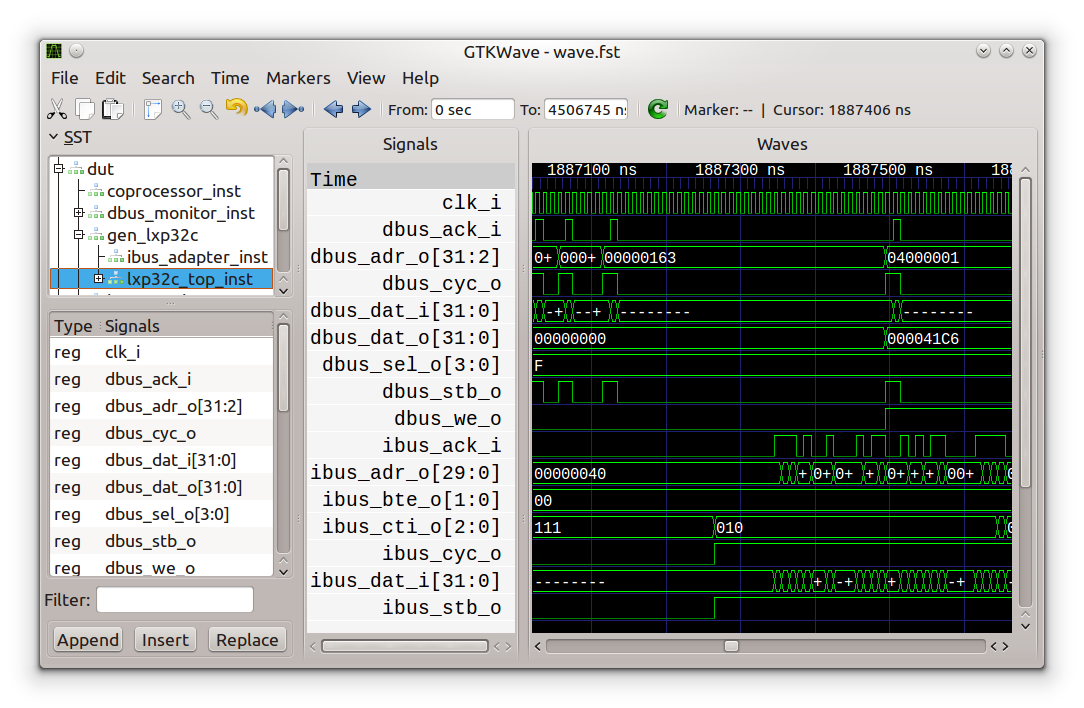
\includegraphics[scale=0.65]{images/gtkwave.png}
	\caption{GTKWave displaying the \lxp{} waveform dump produced by GHDL}
	\label{fig:gtkwave}
\end{figure}

\section{Running simulation using makefiles}

To simulate the design, go to the \shellcmd{verify/lxp32/run/<\emph{simulator}>} directory and run \shellcmd{make}. The following make targets are supported:

\begin{itemize}
	\item \shellcmd{batch} -- simulate the design in batch mode. Results will be written to the standard output. This is the default target.
	\item \shellcmd{gui} -- simulate the design in GUI mode. Note: since GHDL doesn't have a GUI, the simulation itself will be run in batch mode; upon a successful completion, GTKWave will be run automatically to display dumped waveforms.
	\item \shellcmd{compile} -- compile only, don't run simulation.
	\item \shellcmd{clean} -- delete all the produced artifacts.
\end{itemize}

\section{Running simulation manually}
\label{sec:simmanual}

\lxp{} testbench can be also run manually. The following steps must be performed:

\begin{enumerate}
	\item Compile the test firmware in the \shellcmd{verify/lxp32/src/firmware} directory:
	
	\begin{codepar}
    lxp32asm -f textio \emph{filename}.asm -o \emph{filename}.ram
	\end{codepar}
	
	Produced \shellcmd{*.ram} files must be placed to the simulator's working directory.
	\item Compile the \lxp{} RTL description (\shellcmd{rtl} directory).
	\item Compile the common package (\shellcmd{verify/common\_pkg}).
	\item Compile the test platform (\shellcmd{verify/lxp32/src/platform} directory).
	\item Compile the testbench itself (\shellcmd{verify/lxp32/src/tb} directory).
	\item Simulate the \shellcmd{tb} design unit defined in the \shellcmd{tb.vhd} file.
\end{enumerate}

\section{Testbench parameters}

Simulation parameters can be configured by overriding generics defined by the \shellcmd{tb} design unit:

\begin{itemize}
	\item \code{CPU\_DBUS\_RMW} -- \code{DBUS\_RMW} CPU generic value (see Section \ref{sec:generics}).
	\item \code{CPU\_MUL\_ARCH} -- \code{MUL\_ARCH} CPU generic value (see Section \ref{sec:generics}).
	\item \code{MODEL\_LXP32C} -- simulate the \lxp{}C version. By default, this option is set to \code{true}. If set to \code{false}, \lxp{}U is simulated instead.
	\item \code{TEST\_CASE} -- if set to a non-empty string, specifies the file name of a test case to run. If set to an empty string (default), all tests are executed.
	\item \code{THROTTLE\_DBUS} -- perform pseudo-random data bus throttling. By default, this option is set to \code{true}.
	\item \code{THROTTLE\_IBUS} -- perform pseudo-random instruction bus throttling. By default, this option is set to \code{true}.
	\item \code{VERBOSE} -- print more messages.
\end{itemize}

\chapter{Development tools}
\label{ch:developmenttools}

\section{\shellcmd{lxp32asm} -- Assembler and linker}
\label{sec:lxp32asm}

\shellcmd{lxp32asm} is a combined assembler and linker for the \lxp{} platform. It takes one or more input files and produces executable code for the CPU. Input files can be either source files in the \lxp{} assembly language (Appendix \ref{app:assemblylanguage}) or \emph{linkable objects}. Linkable object is a relocatable format for storing compiled \lxp{} code together with symbol information.

\shellcmd{lxp32asm} operates in two stages:

\begin{enumerate}
	\item Compile.
	
	Source files are compiled to linkable objects.
	
	\item Link.
	
	Linkable objects are combined into a single executable module. References to symbols defined in external modules are resolved at this stage.
\end{enumerate}

In the simplest case there is only one input source file which doesn't contain external symbol references. If there are multiple input files, one of them must define the \code{entry} symbol at the beginning of the code.

\subsection{Command line syntax}
\label{subsec:assemblercmdline}

\begin{codepar}
    lxp32asm [ \emph{options} | \emph{input files} ]
\end{codepar}

\subsubsection{General options}

\begin{itemize}
	\item \shellcmd{-c} -- compile only (skip the Link stage).
	
	\item \shellcmd{-h}, \shellcmd{--help} -- display a short help message and exit.
	
	\item \shellcmd{-o \emph{file}} -- output file name.
	
	\item \shellcmd{--} -- do not interpret the subsequent command line arguments as options. Can be used if there are input file names starting with a dash.
\end{itemize}

\subsubsection{Compiler options}

\begin{itemize}
	\item \shellcmd{-i \emph{dir}} -- add \emph{dir} to the list of directories used to search for included files. Multiple directories can be specified with multiple \shellcmd{-i} arguments.
\end{itemize}

\subsubsection{Linker options (ignored in compile-only mode)}

\begin{itemize}
	\item \shellcmd{-a \emph{align}} -- object alignment. Must be a power of 2 and can't be less than 4. Default value is 4.
	
	\item \shellcmd{-b \emph{addr}} -- base address, that is, the address in memory where the executable image will be located. Must be a multiple of object alignment. Default value is 0.
	
	\item \shellcmd{-f \emph{fmt}} -- executable image format. See below for the list of supported formats.
	
	\item \shellcmd{-m \emph{file}} -- generate a map file. A map file is a human-readable list of all object and symbol addresses in the executable image.
	
	\item \shellcmd{-s \emph{size}} -- size of the executable image. Must be a multiple of 4. If total code size is less than the specified value, the executable image is padded with zeros. By default, the image is not padded.
\end{itemize}

\subsection{Output formats}

Output formats that can be specified with the \shellcmd{-f} command line option are listed below.

\begin{itemize}
	\item \shellcmd{bin} -- raw binary image (little-endian). This is the default format.
	\item \shellcmd{textio} -- text format representing binary data as a sequence of zeros and ones. This format can be directly read from VHDL (using the \code{std.textio} package) or Verilog\textregistered{} (using the \code{\$readmemb} function).
	\item \shellcmd{dec} -- text format representing each word as a decimal number.
	\item \shellcmd{hex} -- text format representing each word as a hexadecimal number.
\end{itemize}

\section{\shellcmd{lxp32dump} -- Disassembler}

\shellcmd{lxp32dump} takes an executable image and produces a source file in \lxp{} assembly language. The produced file is a valid program that can be compiled by \shellcmd{lxp32asm}.

\subsection{Command line syntax}

\begin{codepar}
    lxp32dump [ \emph{options} | \emph{input file} ]
\end{codepar}

Supported options are:

\begin{itemize}
	\item \shellcmd{-b \emph{addr}} -- executable image base address, only used for comments.
	
	\item \shellcmd{-f \emph{fmt}} -- input file format. All \shellcmd{lxp32asm} output formats are supported. If this option is not supplied, autodetection is performed.
	
	\item \shellcmd{-h}, \shellcmd{--help} -- display a short help message and exit.
	
	\item \shellcmd{-na} -- do not use instruction aliases (such as \instr{mov}, \instr{ret}, \instr{not}) and register aliases (such as \code{sp}, \code{rp}).
	
	\item \shellcmd{-o \emph{file}} -- output file name. By default, the standard output stream is used.
	
	\item \shellcmd{--} -- do not interpret subsequent command line arguments as options.
\end{itemize}

\section{\shellcmd{wigen} -- Interconnect generator}

\shellcmd{wigen} is a small tool that generates VHDL description of a simple WISHBONE interconnect based on shared bus topology. It supports any number of masters and slaves. The interconnect can then be used to create a SoC based on \lxp{}.

For interconnects with multiple masters a priority-based arbitration circuit is inserted with lower-numbered masters taking precedence. However, when a bus cycle is in progress ([CYC\_O] is asserted by the active master), the arbiter will not interrupt it even if a master with a higher priority level requests bus ownership.

\subsection{Command line syntax}

\begin{codepar}
	wigen [ \emph{option(s)} ] \emph{nm} \emph{ns} \emph{ma} \emph{sa} \emph{ps} [ \emph{pg} ]
\end{codepar}

\begin{itemize}
	\item\shellcmd{\emph{nm}} -- number of masters,
	\item\shellcmd{\emph{ns}} -- number of slaves,
	\item\shellcmd{\emph{ma}} -- master address width,
	\item\shellcmd{\emph{sa}} -- slave address width,
	\item\shellcmd{\emph{ps}} -- port size (8, 16, 32 or 64),
	\item\shellcmd{\emph{pg}} -- port granularity (8, 16, 32 or 64, default: the same as port size).
\end{itemize}

Supported options are:

\begin{itemize}
	\item \shellcmd{-e \emph{entity}} -- name of the design entity (default is \code{"intercon"}).
	
	\item \shellcmd{-h}, \shellcmd{--help} -- display a short help message and exit.
	
	\item \shellcmd{-o \emph{file}} -- output file name (default is \shellcmd{\emph{entity}.vhd}).
	
	\item \shellcmd{-p} -- generate pipelined arbiter (reduced combinatorial delays, increased latency).
	
	\item \shellcmd{-r} -- generate WISHBONE registered feedback signals ([CTI\_IO()] and [BTE\_IO()]).
	
	\item \shellcmd{-u} -- generate unsafe slave decoder (reduced combinatorial delays and resource usage, may not work properly if the address is invalid).
\end{itemize}

\section{Building from source}
\label{sec:buildfromsource}

Prebuilt tool executables for 32-bit Microsoft\textregistered{} Windows\textregistered{} are included in the \lxp{} IP core package. For other platforms the tools must be built from source. Since they are developed in \cplusplus{} using only the standard library, it should be possible to build them for any platform that provides a modern \cplusplus{} compiler.

\subsection{Requirements}

The following software is required to build \lxp{} tools from source:

\begin{enumerate}
	\item A modern \cplusplus{} compiler, such as Microsoft\textregistered{} Visual Studio\textregistered{} 2013 or newer, GCC 4.8 or newer, Clang 3.4 or newer.
	\item CMake 3.3 or newer.
\end{enumerate}

\subsection{Build procedure}

This software uses CMake as a build system generator. Building it involves two steps: first, the \shellcmd{cmake} program is invoked to generate a native build environment (a set of Makefiles or an IDE project); second, the generated environment is used to build the software. More details can be found in the CMake documentation.

\subsubsection{Examples}

In the following examples, it is assumed that the commands are run from the \shellcmd{tools} subdirectory of the \lxp{} IP core package tree.

For Microsoft\textregistered{} Visual Studio\textregistered{}:

\begin{codepar}
    mkdir build
    cd build
    cmake -G "NMake Makefiles" ../src
    nmake
    nmake install
\end{codepar}

For MSYS:

\begin{codepar}
    mkdir build
    cd build
    cmake -G "MSYS Makefiles" ../src
    make
    make install
\end{codepar}

For MinGW without MSYS:

\begin{codepar}
    mkdir build
    cd build
    cmake -G "MinGW Makefiles" ../src
    mingw32-make
    mingw32-make install
\end{codepar}

For other platforms:

\begin{codepar}
    mkdir build
    cd build
    cmake ../src
    make
    make install
\end{codepar}

\appendix

\chapter{Instruction set reference}
\label{app:instructionset}

See Section \ref{sec:instructionformat} for a general description of \lxp{} instruction encoding.

\section{List of instructions by group}

\begin{ctabular}{lll}
	\toprule
	Instruction & Description & Opcode \\
	\midrule
	\tabcutin{3}{Data transfer} \\
	\midrule
	\hyperref[subsec:instr:mov]{\instr{mov}} & Move & alias for \code{\instr{add} dst, src, 0} \\
	\hyperref[subsec:instr:lc]{\instr{lc}} & Load Constant & \code{000001} \\
	\hyperref[subsec:instr:lcs]{\instr{lcs}} & Load Constant Short & \code{101xxx} \\
	\hyperref[subsec:instr:lw]{\instr{lw}} & Load Word & \code{001000} \\
	\hyperref[subsec:instr:lub]{\instr{lub}} & Load Unsigned Byte & \code{001010} \\
	\hyperref[subsec:instr:lsb]{\instr{lsb}} & Load Signed Byte & \code{001011} \\
	\hyperref[subsec:instr:sw]{\instr{sw}} & Store Word & \code{001100} \\
	\hyperref[subsec:instr:sb]{\instr{sb}} & Store Byte & \code{001110} \\
	\midrule
	\tabcutin{3}{Arithmetic operations} \\
	\midrule
	\hyperref[subsec:instr:add]{\instr{add}} & Add & \code{010000} \\
	\hyperref[subsec:instr:sub]{\instr{sub}} & Subtract & \code{010001} \\
	\hyperref[subsec:instr:neg]{\instr{neg}} & Negate & alias for \code{\instr{sub} dst, 0, src} \\
	\hyperref[subsec:instr:mul]{\instr{mul}} & Multiply & \code{010010} \\
	\hyperref[subsec:instr:divu]{\instr{divu}} & Divide Unsigned & \code{010100} \\
	\hyperref[subsec:instr:divs]{\instr{divs}} & Divide Signed & \code{010101} \\
	\hyperref[subsec:instr:modu]{\instr{modu}} & Modulo Unsigned & \code{010110} \\
	\hyperref[subsec:instr:mods]{\instr{mods}} & Modulo Signed & \code{010111} \\
	\midrule
	\tabcutin{3}{Bitwise operations} \\
	\midrule
	\hyperref[subsec:instr:not]{\instr{not}} & Bitwise Not & alias for \code{\instr{xor} dst, src, -1} \\
	\hyperref[subsec:instr:and]{\instr{and}} & Bitwise And & \code{011000} \\
	\hyperref[subsec:instr:or]{\instr{or}} & Bitwise Or & \code{011001} \\
	\hyperref[subsec:instr:xor]{\instr{xor}} & Bitwise Exclusive Or & \code{011010}\\
	\hyperref[subsec:instr:sl]{\instr{sl}} & Shift Left & \code{011100} \\
	\hyperref[subsec:instr:sru]{\instr{sru}} & Shift Right Unsigned & \code{011110} \\
	\hyperref[subsec:instr:srs]{\instr{srs}} & Shift Right Signed & \code{011111} \\
	\midrule
	\tabcutin{3}{Execution transfer} \\
	\midrule
	\hyperref[subsec:instr:jmp]{\instr{jmp}} & Jump & \code{100000} \\
	\hyperref[subsec:instr:cjmpxxx]{\instr{cjmp\emph{xxx}}} & Compare and Jump & \code{11\emph{xxxx}} (\code{\emph{xxxx}} = condition) \\
	\hyperref[subsec:instr:call]{\instr{call}} & Call Procedure & \code{100001} \\
	\hyperref[subsec:instr:ret]{\instr{ret}} & Return from Procedure & alias for \code{\instr{jmp} rp} \\
	\hyperref[subsec:instr:iret]{\instr{iret}} & Interrupt Return & alias for \code{\instr{jmp} irp}\\
	\midrule
	\tabcutin{3}{Miscellaneous instructions} \\
	\midrule
	\hyperref[subsec:instr:nop]{\instr{nop}} & No Operation & \code{000000} \\
	\hyperref[subsec:instr:hlt]{\instr{hlt}} & Halt & \code{000010} \\
\end{ctabular}

\section{Alphabetical list of instructions}

\settocdepth{subsection}

{
\setlength{\parindent}{0pt}
\nonzeroparskip

\subsection{\instr{add} -- Add}
\label{subsec:instr:add}

\subsubsection{Syntax}

\code{\instr{add} DST, RD1, RD2}

\subsubsection{Encoding}

\code{010000 T1 T2 DST RD1 RD2}

Example: \code{\instr{add} r2, r1, 10} $\rightarrow$ \code{0x4202010A}

\subsubsection{Operation}

\code{DST := RD1 + RD2}

\subsection{\instr{and} -- Bitwise And}
\label{subsec:instr:and}

\subsubsection{Syntax}

\code{\instr{and} DST, RD1, RD2}

\subsubsection{Encoding}

\code{011000 T1 T2 DST RD1 RD2}

Example: \code{\instr{and} r2, r1, 0x3F} $\rightarrow$ \code{0x6202013F}

\subsubsection{Operation}

\code{DST := RD1 $\land$ RD2}

\subsection{\instr{call} -- Call Procedure}
\label{subsec:instr:call}

Save a pointer to the next instruction in the \code{rp} register and transfer execution to the address pointed by the operand.

\subsubsection{Syntax}

\code{\instr{call} RD1}

\subsubsection{Encoding}

\code{100001 1 0 11111110 RD1 00000000}

RD1 must be a register.

Example: \code{\instr{call} r1} $\rightarrow$ \code{0x86FE0100}

\subsubsection{Operation}

\code{rp := \emph{return\_address}}

\code{goto RD1}

Pointer in RD1 is interpreted as described in Section \ref{sec:addressing}.

\subsection{\instr{cjmp\emph{xxx}} -- Compare and Jump}
\label{subsec:instr:cjmpxxx}

Compare two operands and transfer execution to the specified address if a condition is satisfied.

\subsubsection{Syntax}

\code{\instr{cjmpe} DST, RD1, RD2} (Equal)

\code{\instr{cjmpne} DST, RD1, RD2} (Not Equal)

\code{\instr{cjmpsg} DST, RD1, RD2} (Signed Greater)

\code{\instr{cjmpsge} DST, RD1, RD2} (Signed Greater or Equal)

\code{\instr{cjmpsl} DST, RD1, RD2} (Signed Less)

\code{\instr{cjmpsle} DST, RD1, RD2} (Signed Less or Equal)

\code{\instr{cjmpug} DST, RD1, RD2} (Unsigned Greater)

\code{\instr{cjmpuge} DST, RD1, RD2} (Unsigned Greater or Equal)

\code{\instr{cjmpul} DST, RD1, RD2} (Unsigned Less)

\code{\instr{cjmpule} DST, RD1, RD2} (Unsigned Less or Equal)

\subsubsection{Encoding}

\code{OPCODE T1 T2 DST RD1 RD2}

Opcodes:

\begin{tabularx}{\textwidth}{lL}
\instr{cjmpe}   & \code{111000} \\
\instr{cjmpne}  & \code{110100} \\
\instr{cjmpsg}  & \code{110001} \\
\instr{cjmpsge} & \code{111001} \\
\instr{cjmpug}  & \code{110010} \\
\instr{cjmpuge} & \code{111010} \\
\end{tabularx}

\instr{cjmpsl}, \instr{cjmpsle}, \instr{cjmpul}, \instr{cjmpule} instructions are aliases for \instr{cjmpsg}, \instr{cjmpsge}, \instr{cjmpug}, \instr{cjmpuge}, respectively, with RD1 and RD2 operands swapped.

Example: \code{\instr{cjmpuge} r2, r1, 5} $\rightarrow$ \code{0xEA020105}

\subsubsection{Operation}

\code{if \emph{condition} then goto DST}

Pointer in DST is interpreted as described in Section \ref{sec:addressing}. Unlike most instructions, \instr{cjmp\emph{xxx}} does not write to DST.

\subsection{\instr{divs} -- Divide Signed}
\label{subsec:instr:divs}

\subsubsection{Syntax}

\code{\instr{divs} DST, RD1, RD2}

\subsubsection{Encoding}

\code{010101 T1 T2 DST RD1 RD2}

Example: \code{\instr{divs} r2, r1, -3} $\rightarrow$ \code{0x560201FD}

\subsubsection{Operation}

\code{DST := (\emph{signed}) RD1 / (\emph{signed}) RD2}

The result is rounded towards zero and is undefined if RD2 is zero. If the CPU was configured without a divider, this instruction returns \code{0}.

\subsection{\instr{divu} -- Divide Unsigned}
\label{subsec:instr:divu}

\subsubsection{Syntax}

\code{\instr{divu} DST, RD1, RD2}

\subsubsection{Encoding}

\code{010100 T1 T2 DST RD1 RD2}

Example: \code{\instr{divu} r2, r1, 73} $\rightarrow$ \code{0x52020107}

\subsubsection{Operation}

\code{DST := RD1 / RD2}

The result is rounded towards zero and is undefined if RD2 is zero. If the CPU was configured without a divider, this instruction returns \code{0}.

\subsection{\instr{hlt} -- Halt}
\label{subsec:instr:hlt}

Wait for an interrupt.

\subsubsection{Syntax}

\code{\instr{hlt}}

\subsubsection{Encoding}

\code{000010 0 0 00000000 00000000 00000000}

\subsubsection{Operation}

Pause execution until an interrupt is received.

\subsection{\instr{jmp} -- Jump}
\label{subsec:instr:jmp}

Transfer execution to the address pointed by the operand.

\subsubsection{Syntax}

\code{\instr{jmp} RD1}

\subsubsection{Encoding}

\code{100000 1 0 00000000 RD1 00000000}

RD1 must be a register.

Example: \code{\instr{jmp} r1} $\rightarrow$ \code{0x82000100}

\subsubsection{Operation}

\code{goto RD1}

Pointer in RD1 is interpreted as described in Section \ref{sec:addressing}.

\subsection{\instr{iret} -- Interrupt Return}
\label{subsec:instr:iret}

Return from an interrupt handler.

\subsubsection{Syntax}

\instr{iret}

Alias for \code{\instr{jmp} irp}.

\subsection{\instr{lc} -- Load Constant}
\label{subsec:instr:lc}

Load a 32-bit word to the specified register. Note that values from the [-1048576; 1048575] range can be loaded more efficiently using the \instr{lcs} instruction.

\subsubsection{Syntax}

\code{\instr{lc} DST, WORD32}

\subsubsection{Encoding}

\code{000001 0 0 DST 00000000 00000000 WORD32}

Unlike other instructions, \instr{lc} occupies two 32-bit words.

Example: \code{\instr{lc} r1, 0x12345678} $\rightarrow$ \code{0x04010000 0x12345678}

\subsubsection{Operation}

\code{DST := WORD32}

\subsection{\instr{lcs} -- Load Constant Short}
\label{subsec:instr:lcs}

Load a signed value from the [-1048576; 1048575] range (a sign extended 21-bit value) to the specified register. Unlike the \instr{lc} instruction, this instruction is encoded as a single word.

\subsubsection{Syntax}

\code{\instr{lcs} DST, VAL}

\subsubsection{Encoding}

\code{101 VAL[20:16] DST VAL[15:0]}

Example: \code{\instr{lcs} r1, -1000000} $\rightarrow$ \code{0xB001BDC0}

\subsubsection{Operation}

\code{DST := (\emph{signed}) VAL}

\subsection{\instr{lsb} -- Load Signed Byte}
\label{subsec:instr:lsb}

Load a byte from the specified address to the register, performing sign extension.

\subsubsection{Syntax}

\code{\instr{lsb} DST, RD1}

\subsubsection{Encoding}

\code{001011 1 0 DST RD1 00000000}

RD1 must be a register.

Example: \code{\instr{lsb} r2, r1} $\rightarrow$ \code{0x2E020100}

\subsubsection{Operation}

\code{DST := (\emph{signed}) (*(BYTE*)RD1)}

Pointer in RD1 is interpreted as described in Section \ref{sec:addressing}.

\subsection{\instr{lub} -- Load Unsigned Byte}
\label{subsec:instr:lub}

Load a byte from the specified address to the register. Higher 24 bits are zeroed.

\subsubsection{Syntax}

\code{\instr{lub} DST, RD1}

\subsubsection{Encoding}

\code{001010 1 0 DST RD1 00000000}

RD1 must be a register.

Example: \code{\instr{lub} r2, r1} $\rightarrow$ \code{0x2A020100}

\subsubsection{Operation}

\code{DST := *(BYTE*)RD1}

Pointer in RD1 is interpreted as described in Section \ref{sec:addressing}.

\subsection{\instr{lw} -- Load Word}
\label{subsec:instr:lw}

Load a word from the specified address to the register.

\subsubsection{Syntax}

\code{\instr{lw} DST, RD1}

\subsubsection{Encoding}

\code{001000 1 0 DST RD1 00000000}

RD1 must be a register.

Example: \code{\instr{lw} r2, r1} $\rightarrow$ \code{0x22020100}

\subsubsection{Operation}

\code{DST := *RD1}

Pointer in RD1 is interpreted as described in Section \ref{sec:addressing}.

\subsection{\instr{mods} -- Modulo Signed}
\label{subsec:instr:mods}

\subsubsection{Syntax}

\code{\instr{mods} DST, RD1, RD2}

\subsubsection{Encoding}

\code{010111 T1 T2 DST RD1 RD2}

Example: \code{\instr{mods} r2, r1, 10} $\rightarrow$ \code{0x5E02010A}

\subsubsection{Operation}

\code{DST := (\emph{signed}) RD1 mod (\emph{signed}) RD2}

Modulo operation satisfies the following condition: if $Q=A/B$ and $R=A \mod B$, then $A=B \cdot Q+R$.

The result is undefined if RD2 is zero. If the CPU was configured without a divider, this instruction returns \code{0}.

\subsection{\instr{modu} -- Modulo Unsigned}
\label{subsec:instr:modu}

\subsubsection{Syntax}

\code{\instr{modu} DST, RD1, RD2}

\subsubsection{Encoding}

\code{010110 T1 T2 DST RD1 RD2}

Example: \code{\instr{modu} r2, r1, 10} $\rightarrow$ \code{0x5A02010A}

\subsubsection{Operation}

\code{DST := RD1 mod RD2}

Modulo operation satisfies the following condition: if $Q=A/B$ and $R=A \mod B$, then $A=B \cdot Q+R$.

The result is undefined if RD2 is zero. If the CPU was configured without a divider, this instruction returns \code{0}.

\subsection{\instr{mov} -- Move}
\label{subsec:instr:mov}

\subsubsection{Syntax}

\code{\instr{mov} DST, RD1}

Alias for \code{\instr{add} DST, RD1, 0}

\subsection{\instr{mul} -- Multiply}
\label{subsec:instr:mul}

Multiply two 32-bit values. The result is also 32-bit.

\subsubsection{Syntax}

\code{\instr{mul} DST, RD1, RD2}

\subsubsection{Encoding}

\code{010010 T1 T2 DST RD1 RD2}

Example: \code{\instr{mul} r2, r1, 3} $\rightarrow$ \code{0x4A020103}

\subsubsection{Operation}

\code{DST := RD1 * RD2}

Since the product width is the same as the operand width, the result of a multiplication does not depend on operand signedness.

\subsection{\instr{neg} -- Negate}
\label{subsec:instr:neg}

\subsubsection{Syntax}

\code{\instr{neg} DST, RD2}

Alias for \code{\instr{sub} DST, 0, RD2}

\subsection{\instr{nop} -- No Operation}
\label{subsec:instr:nop}

\subsubsection{Syntax}

\instr{nop}

\subsubsection{Encoding}

\code{000000 0 0 00000000 00000000 00000000}

\subsubsection{Operation}

This instruction does not alter the machine state.

\subsection{\instr{not} -- Bitwise Not}
\label{subsec:instr:not}

\subsubsection{Syntax}

\code{\instr{not} DST, RD1}

Alias for \code{\instr{xor} DST, RD1, -1}.

\subsection{\instr{or} -- Bitwise Or}
\label{subsec:instr:or}

\subsubsection{Syntax}

\code{\instr{or} DST, RD1, RD2}

\subsubsection{Encoding}

\code{011001 T1 T2 DST RD1 RD2}

Example: \code{\instr{or} r2, r1, 0x3F} $\rightarrow$ \code{0x6602013F}

\subsubsection{Operation}

\code{DST := RD1 $\lor$ RD2}

\subsection{\instr{ret} -- Return from Procedure}
\label{subsec:instr:ret}

Return from a procedure.

\subsubsection{Syntax}

\instr{ret}

Alias for \code{\instr{jmp} rp}.

\subsection{\instr{sb} -- Store Byte}
\label{subsec:instr:sb}

Store the lowest byte from the register to the specified address.

\subsubsection{Syntax}

\code{\instr{sb} RD1, RD2}

\subsubsection{Encoding}

\code{001110 1 T2 00000000 RD1 RD2}

RD1 must be a register.

Example: \code{\instr{sb} r2, r1} $\rightarrow$ \code{0x3B000201}

\subsubsection{Operation}

\code{*(BYTE*)RD1 := RD2 $\land$ 0x000000FF}

Pointer in RD1 is interpreted as described in Section \ref{sec:addressing}.

\subsection{\instr{sl} -- Shift Left}
\label{subsec:instr:sl}

\subsubsection{Syntax}

\code{\instr{sl} DST, RD1, RD2}

\subsubsection{Encoding}

\code{011100 T1 T2 DST RD1 RD2}

Example: \code{\instr{sl} r2, r1, 5} $\rightarrow$ \code{0x72020105}

\subsubsection{Operation}

\code{DST := RD1 << RD2}

The result is undefined if RD2 is outside the [0; 31] range.

\subsection{\instr{srs} -- Shift Right Signed}
\label{subsec:instr:srs}

\subsubsection{Syntax}

\code{\instr{srs} DST, RD1, RD2}

\subsubsection{Encoding}

\code{011111 T1 T2 DST RD1 RD2}

Example: \code{\instr{srs} r2, r1, 5} $\rightarrow$ \code{0x7E020105}

\subsubsection{Operation}

\code{DST := ((\emph{signed}) RD1) >> RD2}

The result is undefined if RD2 is outside the [0; 31] range.

\subsection{\instr{sru} -- Shift Right Unsigned}
\label{subsec:instr:sru}

\subsubsection{Syntax}

\code{\instr{sru} DST, RD1, RD2}

\subsubsection{Encoding}

\code{011110 T1 T2 DST RD1 RD2}

Example: \code{\instr{sru} r2, r1, 5} $\rightarrow$ \code{0x7A020105}

\subsubsection{Operation}

\code{DST := RD1 >> RD2}

The result is undefined if RD2 is outside the [0; 31] range.

\subsection{\instr{sub} -- Subtract}
\label{subsec:instr:sub}

\subsubsection{Syntax}

\code{\instr{sub} DST, RD1, RD2}

\subsubsection{Encoding}

\code{010001 T1 T2 DST RD1 RD2}

Example: \code{\instr{sub} r2, r1, 5} $\rightarrow$ \code{0x46020105}

\subsubsection{Operation}

\code{DST := RD1 - RD2}

\subsection{\instr{sw} -- Store Word}
\label{subsec:instr:sw}

Store the value of the register to the specified address.

\subsubsection{Syntax}

\code{\instr{sw} RD1, RD2}

\subsubsection{Encoding}

\code{001100 1 T2 00000000 RD1 RD2}

RD1 must be a register.

Example: \code{\instr{sw} r2, r1} $\rightarrow$ \code{0x33000201}

\subsubsection{Operation}

\code{*RD1 := RD2}

Pointer in RD1 is interpreted as described in Section \ref{sec:addressing}.

\subsection{\instr{xor} -- Bitwise Exclusive Or}
\label{subsec:instr:xor}

\subsubsection{Syntax}

\code{\instr{xor} DST, RD1, RD2}

\subsubsection{Encoding}

\code{011010 T1 T2 DST RD1 RD2}

Example: \code{\instr{xor} r2, r1, 0x3F} $\rightarrow$ \code{0x6A02013F}

\subsubsection{Operation}

\code{DST := RD1 $\oplus$ RD2}

}

\settocdepth{section}

\chapter{Instruction cycle counts}

Cycle counts for \lxp{} instructions are listed in Table \ref{tab:cycles}, based on an assumption that no pipeline stalls are caused by the instruction bus latency or cache misses. These data are provided for reference purposes; the software should not depend on them as they can change in future hardware revisions.

\begin{table}[htbp]
	\centering
	\caption{Instruction cycle counts}
	\label{tab:cycles}
	\begin{tabularx}{0.8\textwidth}{LLLL}
		\toprule
		Instruction & Cycles & Instruction & Cycles \\
		\midrule
		\instr{add} & 1 & \instr{modu} & 37 \\
		\instr{and} & 1 & \instr{mov} & 1 \\
		\instr{call} & 4 & \instr{mul} & 2, 6 or 34\footnotemark[3] \\
		\instr{cjmp\emph{xxx}} & 5 or 2\footnotemark[1] & \instr{neg} & 1 \\
		\instr{divs} & 36 & \instr{nop} & 1 \\
		\instr{divu} & 36 & \instr{not} & 1 \\
		\instr{hlt} & N/A & \instr{or} & 1 \\
		\instr{jmp} & 4 & \instr{ret} & 4 \\
		\instr{iret} & 4 & \instr{sb} & $\ge$ 2\footnotemark[2] \\
		\instr{lc} & 2 & \instr{sl} & 2 \\
		\instr{lcs} & 1 & \instr{srs} & 2 \\
		\instr{lsb} & $\ge$ 3\footnotemark[2] & \instr{sru} & 2 \\
		\instr{lub} & $\ge$ 3\footnotemark[2] & \instr{sub} & 1 \\
		\instr{lw} & $\ge$ 3\footnotemark[2] & \instr{sw} & $\ge$ 2\footnotemark[2] \\
		\instr{mods} & 37 & \instr{xor} & 1 \\
		\bottomrule
	\end{tabularx}
\end{table}

\footnotetext[1]{Depends on whether the jump is taken or not.}
\footnotetext[2]{Depends on the data bus latency.}
\footnotetext[3]{Depends on the multiplier architecture. See Section \ref{sec:generics}.}

\chapter{LXP32 assembly language}
\label{app:assemblylanguage}

This appendix defines the assembly language used by \lxp{} development tools.

\section{Comments}

\lxp{} assembly language supports C style comments that can span across multiple lines and single-line \cplusplus{} style comments:

\begin{codepar}\itshape
    /*
     * This is a comment.
     */

    // This is also a comment
\end{codepar}

From a parser's point of view comments are equivalent to whitespace.

\section{Literals}

\lxp{} assembly language uses numeric and string literals similar to those provided by the C programming language.

Numeric literals can take form of decimal, hexadecimal or octal numbers. Literals prefixed with \code{0x} are interpreted as hexadecimal, literals prefixed with \code{0} are interpreted as octal, other literals are interpreted as decimal. A numeric literal can also start with an unary plus or minus sign which is also considered a part of the literal.

String literals must be enclosed in double quotes. The most common escape sequences used in C are supported (Table \ref{tab:stringescape}). Note that strings are not null-terminated in the LXP32 assembly language; when required, terminating null character must be inserted explicitly.

\begin{table}[htbp]
	\caption{Escape sequences used in string literals}
	\label{tab:stringescape}
	\begin{tabularx}{\textwidth}{lL}
		\toprule
		Sequence & Interpretation \\
		\midrule
		\code{\textbackslash\textbackslash} & Backslash character \\
		\code{\textbackslash "} & Double quotation mark \\
		\code{\textbackslash '} & Single quotation mark (can be also used directly) \\
		\code{\textbackslash t} & Tabulation character \\
		\code{\textbackslash n} & Line feed \\
		\code{\textbackslash r} & Carriage return \\
		\code{\textbackslash x\emph{XX}} & Character with a hexadecimal code of \emph{XX} (1--2 digits) \\
		\code{\textbackslash \emph{XXX}} & Character with an octal code of \emph{XXX} (1--3 digits) \\
		\bottomrule
	\end{tabularx}
\end{table}

\section{Symbols}
\label{sec:symbols}

Symbols (labels) are used to refer to data or code locations. \lxp{} assembly language does not have distinct code and data labels: symbols are used in both these contexts.

Symbol names must be valid identifiers. A valid identifier must start with an alphabetic character or an underscore, and may contain alphanumeric characters and underscores.

A symbol definition must be the first token in a source code line followed by a colon. A symbol definition can occupy a separate line (in which case it refers to the following statement). Alternatively, a statement can follow the symbol definition on the same line.

Symbols can be used as operands to the \instr{lc} and \instr{lcs} instruction statements. A symbol reference can end with a \code{@\emph{n}} sequence, where \code{\emph{n}} is a numeric literal; in this case it is interpreted as an offset (in bytes) relative to the symbol definition. For the \instr{lcs} instruction, the resulting address must still fit into the sign extended 21-bit value range (\code{0x00000000}--\code{0x000FFFFF} or \code{0xFFF00000}--\code{0xFFFFFFFF}), otherwise the linker will report an error.

By default all symbols are local, that is, they can be only referenced from the module where they were defined. To make a symbol accessible from other modules, use the \instr{\#export} directive. To reference a symbol defined in another module use the \instr{\#import} directive.

A symbol named \code{entry} or \code{Entry} has a special meaning: it is used to inform the linker about the program entry point if there are multiple input files. It does not have to be exported. If defined, this symbol must precede the first instruction or data definition statement in the module. Only one module in the program can define the entry symbol.

\begin{codeparbreakable}
    \instr{lc} r10, jump\_label
    \instr{lc} r11, data\_word
\emph{// ...}
    \instr{sw} r11, r0 \emph{// store the value of r0 to the}
               \emph{// location pointed by data\_word}
    \instr{jmp} r10    \emph{// transfer execution to jump\_label}
\emph{// ...}
jump\_label:
    \instr{mov} r1, r0
\emph{// ...}
data\_word:
    \instr{.word} 0x12345678
\end{codeparbreakable}

\section{Statements}

Each statement occupies a single source code line. There are three kinds of statements:

\begin{itemize}
	\item \emph{Directives} provide directions for the assembler that do not directly cause code generation.
	\item \emph{Data definition statements} insert arbitrary data to the generated code.
	\item \emph{Instruction statements} insert \lxp{} CPU instructions to the generated code.
\end{itemize}

\subsection{Directives}

The first token of a directive statement always starts with the \code{\#} character.

\begin{codepar}
\instr{\#define} \emph{identifier} \emph{token} [ \emph{token} ... ]
\end{codepar}

Defines a macro that will be substituted with one or more tokens. The \code{\emph{identifier}} must satisfy the requirements listed in Section \ref{sec:symbols}. Tokens can be anything, including keywords, identifiers, literals and separators (i.e. comma and colon characters).

\begin{codepar}
\instr{\#export} \emph{identifier}
\end{codepar}

Declares \code{\emph{identifier}} as an exported symbol. Exported symbols can be referenced by other modules.

\begin{codepar}
\instr{\#import} \emph{identifier}
\end{codepar}

Declares \code{\emph{identifier}} as an imported symbol. Used to refer to symbols exported by other modules.

\begin{codepar}
\instr{\#include} \emph{filename}
\end{codepar}

Processes \code{\emph{filename}} contents as it were literally inserted at the point of the \instr{\#include} directive. \code{\emph{filename}} must be a string literal.

\begin{codepar}
\instr{\#message} \emph{msg}
\end{codepar}

Prints \code{\emph{msg}} to the standard output stream. \code{\emph{msg}} must be a string literal.

\subsection{Data definition statements}

The first token of a data definition statement always starts with the \code{.} (period) character.

\begin{codepar}
\instr{.align} [ \emph{alignment} ]
\end{codepar}

Ensures that code generated by the next data definition or instruction statement is aligned to a multiple of \code{\emph{alignment}} bytes, inserting padding zeros if needed. \code{\emph{alignment}} must be a power of 2 and can't be less than 4. Default \code{\emph{alignment}} is 4. Instructions and words are always at least word-aligned; the \instr{.align} statement can be used to align them to a larger boundary, or to align byte data (see below).

The \instr{.align} statement is not guaranteed to work if the requested alignment is greater than the section alignment specified for the linker (see Subsection \ref{subsec:assemblercmdline}).

\begin{codepar}
\instr{.byte} \emph{token} [, \emph{token} ... ]
\end{codepar}

Inserts one or more bytes to the output code. Each \code{\emph{token}} can be either a numeric literal with a valid range of [-128; 255] or a string literal. By default, bytes are not aligned.

To define a null-terminated string, the terminating null character must be inserted explicitly.

\begin{codepar}
\instr{.reserve} \emph{n}
\end{codepar}

Inserts \code{\emph{n}} zero bytes to the output code.

\begin{codepar}
\instr{.word} \emph{token} [, \emph{token} ... ]
\end{codepar}

Inserts one or more 32-bit words to the output code. Tokens must be numeric literals.

\subsection{Instruction statements}

Instruction statements have the following general syntax:

\begin{codepar}
    \instr{\emph{instruction}} [ \emph{operand} [, \emph{operand} ... ] ]
\end{codepar}

Depending on the instruction, operands can be registers, numeric literals or symbols. Supported instructions are listed in Appendix \ref{app:instructionset}.

\chapter{WISHBONE datasheet}
\label{app:wishbonedatasheet}

\section[Instruction bus (LXP32C only)]{Instruction bus (\lxp{}C only)}

\begin{ctabular}{ll}
	\toprule
	\tabcutin{2}{\makebox[0.9\textwidth][c]{General information}} \\
	\midrule
	WISHBONE revision & B3 \\
	Type of interface & MASTER \\
	Supported cycles  & BLOCK READ \\
	\midrule
	\tabcutin{2}{Signal names} \\
	\midrule
	\signal{clk\_i}       & CLK\_I \\
	\signal{rst\_i}       & RST\_I \\
	\signal{ibus\_cyc\_o} & CYC\_O \\
	\signal{ibus\_stb\_o} & STB\_O \\
	\signal{ibus\_cti\_o} & CTI\_O() \\
	\signal{ibus\_bte\_o} & BTE\_O() \\
	\signal{ibus\_ack\_i} & ACK\_I \\
	\signal{ibus\_adr\_o} & ADR\_O() \\
	\signal{ibus\_dat\_i} & DAT\_I() \\
	\midrule
	\tabcutin{2}{Supported tag signals} \\
	\midrule
	\signal{ibus\_cti\_o} & Cycle Type Identifier (address tag) \\
	& \hspace{\parindent} ``010'' (Incrementing burst cycle) \\
	& \hspace{\parindent} ``111'' (End-of-Burst) \\
	\signal{ibus\_bte\_o} & Burst Type Extension (address tag) \\
	& \hspace{\parindent} ``00'' (Linear burst) \\
	\midrule
	\tabcutin{2}{Dimensions} \\
	\midrule
	Port size & 32 \\
	Port granularity & 32 \\
	Maximum operand size & 32 \\
	Data transfer ordering & BIG/LITTLE ENDIAN \\
	Data transfer sequence & UNDEFINED \\
	\bottomrule
\end{ctabular}

\section{Data bus}

\begin{ctabular}{ll}
	\toprule
	\tabcutin{2}{\makebox[0.9\textwidth][c]{General information}} \\
	\midrule
	WISHBONE revision & B3 \\
	Type of interface & MASTER \\
	Supported cycles  & SINGLE READ/WRITE \\
	                  & RMW \\
	\midrule
	\tabcutin{2}{Signal names} \\
	\midrule
	\signal{clk\_i}       & CLK\_I \\
	\signal{rst\_i}       & RST\_I \\
	\signal{dbus\_cyc\_o} & CYC\_O \\
	\signal{dbus\_stb\_o} & STB\_O \\
	\signal{dbus\_we\_o}  & WE\_O \\
	\signal{dbus\_sel\_o} & SEL\_O() \\
	\signal{dbus\_ack\_i} & ACK\_I \\
	\signal{dbus\_adr\_o} & ADR\_O() \\
	\signal{dbus\_dat\_o} & DAT\_O() \\
	\signal{dbus\_dat\_i} & DAT\_I() \\
	\midrule
	\tabcutin{2}{Dimensions} \\
	\midrule
	Port size & 32 \\
	Port granularity & 8 \\
	Maximum operand size & 32 \\
	Data transfer ordering & LITTLE ENDIAN \\
	Data transfer sequence & UNDEFINED \\
	\bottomrule
\end{ctabular}

\chapter{List of changes}

\section*{Version 1.1 (2019-01-11)}

This release introduces a minor but technically breaking hardware change: the START\_ADDR generic, which used to be 30-bit, has been for convenience extended to a full 32-bit word; the two least significant bits are ignored.

The other breaking change affects the assembly language syntax. Previously all symbols used to be public, and multiple modules could not define symbols with the same name. As of now only symbols explicitly exported using the \instr{\#export} directive are public. \instr{\#extern} directive has been replaced by \instr{\#import}.

Other notable changes include:

\begin{itemize}
	\item A new instruction, \instr{lcs} (\instrname{Load Constant Short}), has been added, which loads a 21-bit sign extended constant to a register. Unlike \instr{lc}, it is encoded as a single word and takes one cycle to execute.
	\item Optimizations in the divider unit. Division instructions (\instr{divs} and \instr{divu}) now take one fewer cycle to execute (modulo instructions are unaffected).
	\item LXP32 assembly language now supports a new instruction alias, \instr{neg} (\instrname{Negate}), which is equivalent to \code{\instr{sub} dst, 0, src}.
\end{itemize}

\section*{Version 1.0 (2016-02-20)}

Initial public release.

\end{document}
